%%
%% This is file `sample-sigconf-authordraft.tex',
%% generated with the docstrip utility.
%%
%% The original source files were:
%%
%% samples.dtx  (with options: `all,proceedings,bibtex,authordraft')
%% 
%% IMPORTANT NOTICE:
%% 
%% For the copyright see the source file.
%% 
%% Any modified versions of this file must be renamed
%% with new filenames distinct from sample-sigconf-authordraft.tex.
%% 
%% For distribution of the original source see the terms
%% for copying and modification in the file samples.dtx.
%% 
%% This generated file may be distributed as long as the
%% original source files, as listed above, are part of the
%% same distribution. (The sources need not necessarily be
%% in the same archive or directory.)
%%
%%
%% Commands for TeXCount
%TC:macro \cite [option:text,text]
%TC:macro \citep [option:text,text]
%TC:macro \citet [option:text,text]
%TC:envir table 0 1
%TC:envir table* 0 1
%TC:envir tabular [ignore] word
%TC:envir displaymath 0 word
%TC:envir math 0 word
%TC:envir comment 0 0
%%
%%
%% The first command in your LaTeX source must be the \documentclass
%% command.
%%
%% For submission and review of your manuscript please change the
%% command to \documentclass[manuscript, screen, review]{acmart}.
%%
%% When submitting camera ready or to TAPS, please change the command
%% to \documentclass[sigconf]{acmart} or whichever template is required
%% for your publication.
%%
%%
\documentclass[sigconf,authordraft]{acmart}

%%
%% \BibTeX command to typeset BibTeX logo in the docs
\AtBeginDocument{%
  \providecommand\BibTeX{{%
    Bib\TeX}}}

%% Rights management information.  This information is sent to you
%% when you complete the rights form.  These commands have SAMPLE
%% values in them; it is your responsibility as an author to replace
%% the commands and values with those provided to you when you
%% complete the rights form.
\setcopyright{acmlicensed}
\copyrightyear{2018}
\acmYear{2018}
\acmDOI{1234.7777}

%% These commands are for a PROCEEDINGS abstract or paper.
\acmConference[HCI]{Advanced topics in human-computer interaction}{02 August 2024}{Charlottenburg, B}
%%
%%  Uncomment \acmBooktitle if the title of the proceedings is different
%%  from ``Proceedings of ...''!
%%
%%\acmBooktitle{Woodstock '18: ACM Symposium on Neural Gaze Detection,
%%  June 03--05, 2018, Woodstock, NY}
\acmISBN{123-4-5678-7777-8/02/24}


%%
%% For managing citations, it is recommended to use bibliography
%% files in BibTeX format.
%%
%% You can then either use BibTeX with the ACM-Reference-Format style,
%% or BibLaTeX with the acmnumeric or acmauthoryear sytles, that include
%% support for advanced citation of software artefact from the
%% biblatex-software package, also separately available on CTAN.
%%
%% Look at the sample-*-biblatex.tex files for templates showcasing
%% the biblatex styles.
%%

%%
%% The majority of ACM publications use numbered citations and
%% references.  The command \citestyle{authoryear} switches to the
%% "author year" style.
%%
%% If you are preparing content for an event
%% sponsored by ACM SIGGRAPH, you must use the "author year" style of
%% citations and references.
%% Uncommenting
%% the next command will enable that style.
%%\citestyle{acmauthoryear}


%%
%% end of the preamble, start of the body of the document source.
\begin{document}

%%
%% The "title" command has an optional parameter,
%% allowing the author to define a "short title" to be used in page headers.
\title{Safe Screenshot Capture: Real-Time Privacy Protection for VR/AR}


\author{Ravil Goetzke}
\email{r.goetzke@tu-berln.de}
\affiliation{%
  \institution{Technische Universität}
  \city{Berlin}
  \country{Germany}
}

%%
%% By default, the full list of authors will be used in the page
%% headers. Often, this list is too long, and will overlap
%% other information printed in the page headers. This command allows
%% the author to define a more concise list
%% of authors' names for this purpose.
\renewcommand{\shortauthors}{Goetzke}

%%
%% The abstract is a short summary of the work to be presented in the
%% article.
\begin{abstract}
With the widespread use of augmented reality (AR) and virtual reality (VR) technologies, screenshots are being shared more and more frequently. However, these could contain private content without people being aware of it. This paper introduces a novel system, Safe Screenshot Capture, which enables real-time detection and obfuscation of personal data in a VR environment to enhance privacy protection. The system aims to increase user awareness of the potential dangers of sharing personal data through digital interfaces. This work is grounded in the principles of Human-Computer Interaction (HCI), focusing on user-centered design and iterative development to ensure usability and effectiveness. Initial results indicate that Safe Screenshot Capture significantly heightens user awareness and provides robust privacy protection. However, an unexpected finding was that users tended to rely heavily on the system for privacy management when it functioned effectively. Therefore, this work highlights important implications for the development of privacy-preserving technologies in immersive environments.

  
\end{abstract}

%%
%% The code below is generated by the tool at http://dl.acm.org/ccs.cfm.
%% Please copy and paste the code instead of the example below.
%%
\begin{CCSXML}
<ccs2012>
<concept>
<concept_id>10003120.10003121.10003129.10011757</concept_id>
<concept_desc>Human-centered computing~User interface toolkits</concept_desc>
<concept_significance>500</concept_significance>
</concept>
</ccs2012>
\end{CCSXML}

\ccsdesc[500]{Human-centered computing~User interface toolkits}

% \ccsdesc[500]{Do Not Use This Code~Generate the Correct Terms for Your Paper}
% \ccsdesc[300]{Do Not Use This Code~Generate the Correct Terms for Your Paper}
% \ccsdesc{Do Not Use This Code~Generate the Correct Terms for Your Paper}
% \ccsdesc[100]{Do Not Use This Code~Generate the Correct Terms for Your Paper}

%%
%% Keywords. The author(s) should pick words that accurately describe
%% the work being presented. Separate the keywords with commas.
\keywords{
Human-Computer Interaction, Privacy, Augmented Reality, Virtual Reality, User Privacy, Data Obfuscation, System Usability Scale, Real-time Detection, Immersive Environments, Machine Learning, Privacy Awareness
}

%% A "teaser" image appears between the author and affiliation
%% information and the body of the document, and typically spans the
%% page.
\begin{teaserfigure}
  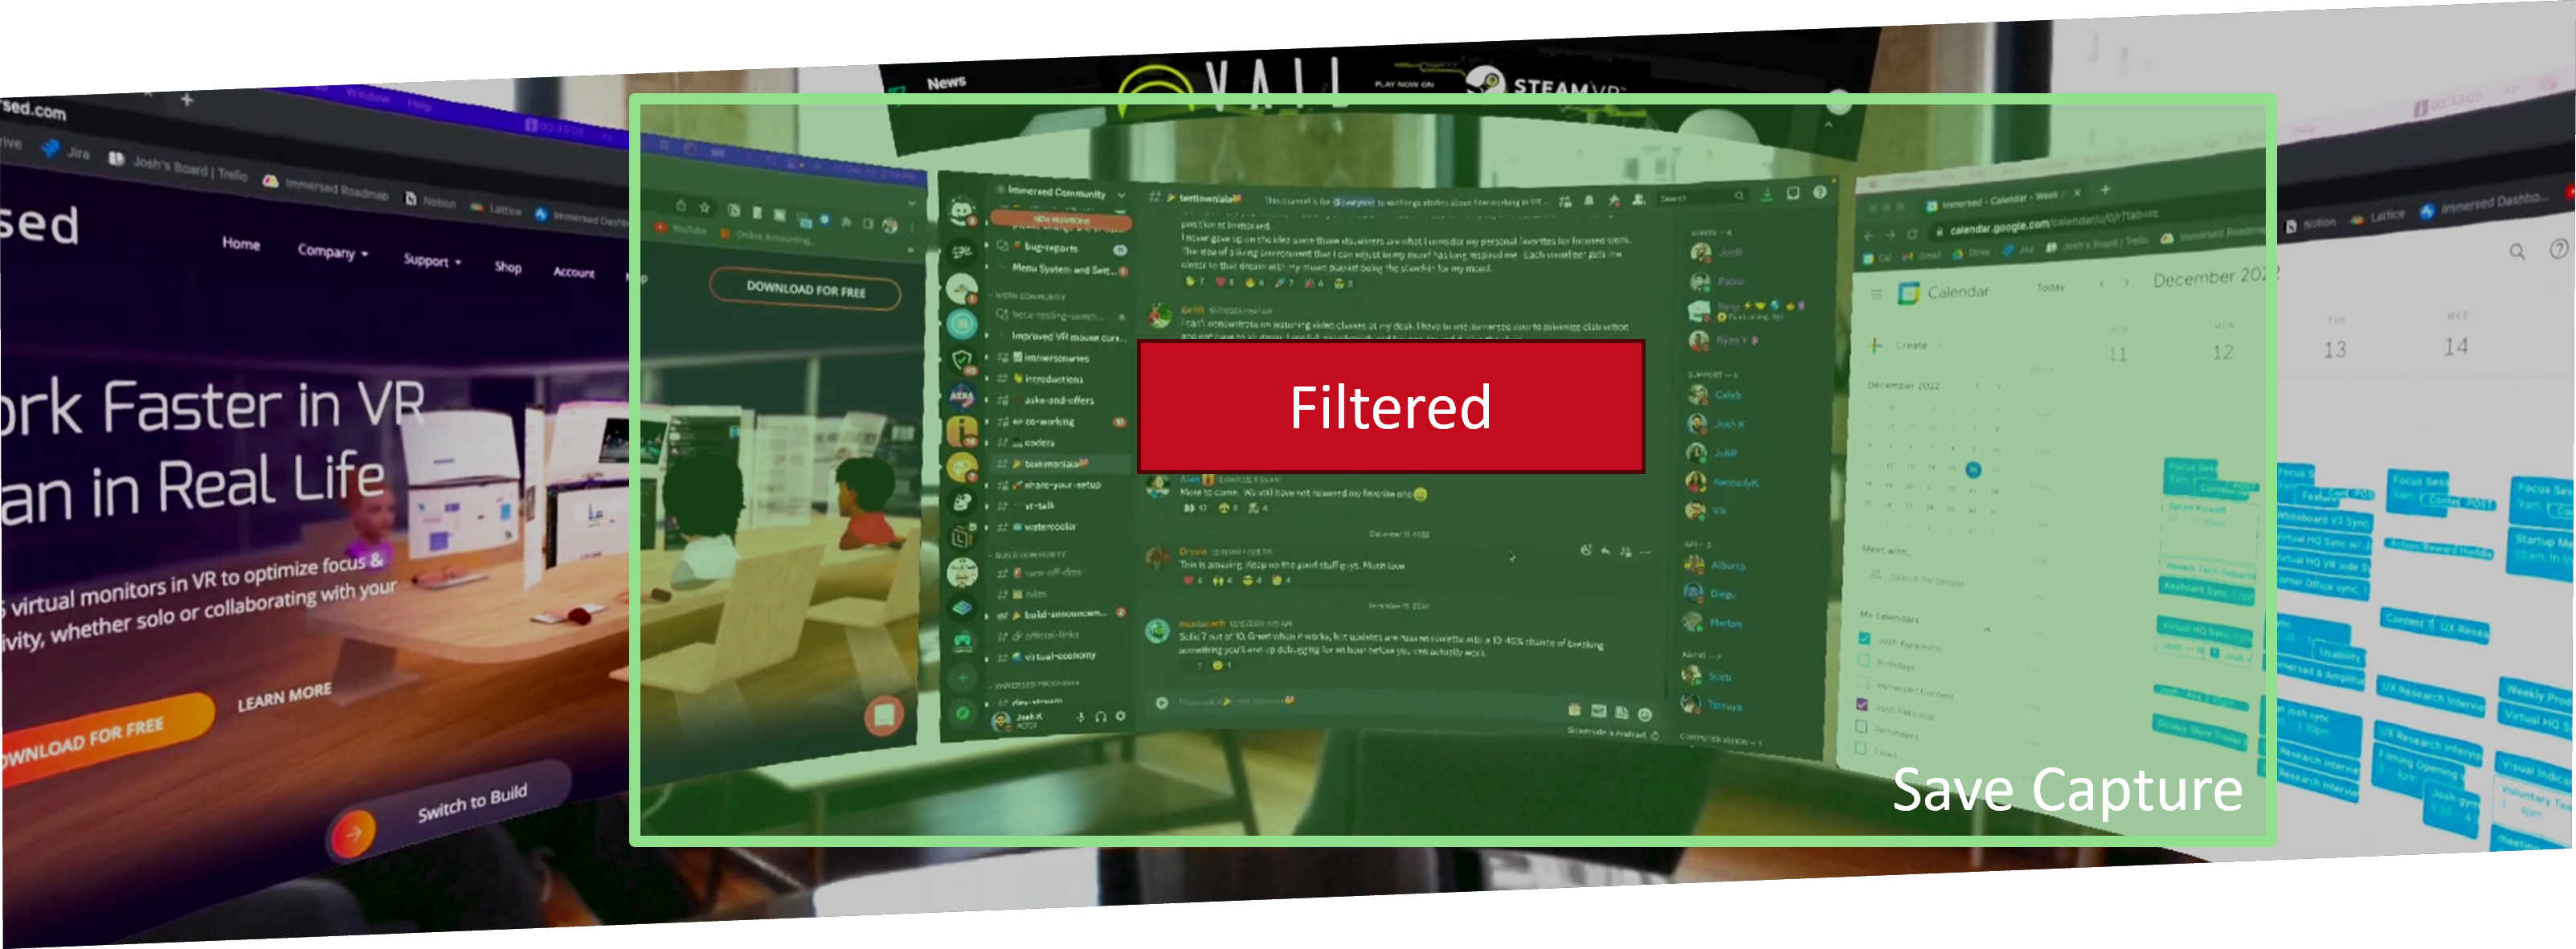
\includegraphics[width=\textwidth]{Teaser.png}
  \caption{Securing Sensitive Information - Auto-Filtered Screenshot in a AR Workspace}
  \Description{Securing Sensitive Information - Auto-Filtered Screenshot in a AR Workspace}
  \label{fig:teaser}
\end{teaserfigure}

\received{02 August 2024}

%%
%% This command processes the author and affiliation and title
%% information and builds the first part of the formatted document.
\maketitle

\section{Introduction}

Augmented reality (AR) and virtual reality (VR) technologies are now widely used, resulting in the frequent sharing of screenshots that may contain sensitive information. This trend reveals a significant gap in tools that can detect and anonymize private data before these images are stored or shared.

Existing systems, such as those developed by Guzman et al. \cite{guzman2023privacy}, have made strides in addressing data protection in mixed realities. However, there is still a lack of practical, user-friendly solutions specifically focused on real-time screenshot privacy. This underscores the urgent need for viable tools that offer effective and intuitive control over personal data in AR and VR environments.

This paper introduces "Safe Screenshot Capture," a novel system designed to enhance privacy by scanning and obfuscating personal information in screenshots. The development of "Safe Screenshot Capture" is anchored in the principles of human-computer interaction (HCI), with a focus on user-centered design and iterative development to create an intuitive and effective privacy protection tool. The system not only shows how to protects privacy but also raises awareness about the potential risks of taking images with personal information inside.

Initial findings demonstrate that "Safe Screenshot Capture" significantly enhances user awareness and provides robust privacy protection in the given VR setting. These outcomes suggest important implications for digital privacy, emphasizing the necessity for ongoing advancements in privacy protection technologies \cite{distler2020how}.

\section{Related Work}
The development of "Safe Screenshot Capture" was significantly influenced by previous work in data protection and security in mixed reality (MR) and user-centered approaches to handling sensitive information in digital interactions.

\subsection{Trade-offs in Privacy}
Users of MR applications frequently take and share pictures of their surroundings \cite{li2024omniactions}. Li et al. \cite{li2024omniactions} developed the OmniActions system, which predicts digital actions in response to real-world multimodal sensory input using large language models (LLMs) \cite{li2024omniactions}. Their diary study with 39 participants found that 65\% regularly took photos to react to or share later, highlighting the need for privacy-compliant systems.

Distler et al. \cite{distler2020how} explored privacy trade-offs in a focus group study with 32 participants. They found that 78\% of participants felt more comfortable using technology that provided clear control over their data, suggesting that real-time filtering of sensitive data could increase user trust and acceptance.

\subsection{Privacy Concerns in Immersive Environments}
Privacy concerns are heightened in immersive environments like VR and AR \cite{adams2018ethics}. Adams et al. \cite{adams2018ethics} interviewed 20 VR users and developers, finding significant privacy concerns and a notable gap in transparency, with only 30\% of VR apps having a privacy policy, and only 19\% mentioning VR-specific data. This lack of transparency contributes to user discomfort and mistrust.

Guzman et al. highlighted the potential for attackers to exploit data collected by MR systems, as these often send large amounts of data to remote servers, posing privacy risks if hacked. Their analysis emphasized the need for robust privacy protection mechanisms in real time.

\subsection{Solutions for Protecting Privacy}
Several methods have been proposed to protect user data in immersive environments \cite{guzman2023privacy}. Guzman et al. discussed intermediary protection mechanisms that filter sensitive data before storage or transmission, emphasizing the importance of real-time filtering to hide private information.

One method presented by Guzman et al. involved conservative layer sharing to protect spatial privacy, effectively reducing the risk of spatial inference attacks while preserving data utility for MR applications \cite{guzman2023privacy}. Despite these advancements, they identified the need for continued research to develop comprehensive privacy protection strategies as MR devices and services evolve.


\section{Implementation}

The "Safe Screenshot Capture" Application was developed using Unity (2022.3.12f1) and an Oculus Quest 3. The XR Interaction Toolkit\footnote{\url{https://docs.unity3d.com/Packages/com.unity.xr.interaction.toolkit@3.0}} was utilized throughout all versions of the development process.

\subsection{Initial Setup and Exploration}
The development process began with familiarization with Unity and the XR Interaction Toolkit. Due to Meta's restriction on accessing passthrough camera data, the "Hands Interaction Demo" sample scene was used. A simple window was created in the user’s view to represent the screenshot area, which could be toggled via hand controllers. Screenshots were captured using the main camera and saved to the \texttt{persistentDataPath}.
\begin{figure}[h]
  \centering
  \includegraphics[width=0.9\linewidth]{Office.png}
  \caption{VR office environment used in the latest version}
  \label{fig:office_environment}
\end{figure}
\subsection{First Iteration}
Initial user testing revealed that the interface was cumbersome and unclear. Users found the App unhandy and bulky, prompting a redesign.

\subsection{Development of Test Scenario}
A new scene was created, simulating a cluttered office - a similar to figure \ref{fig:office_environment} - with objects tagged as \texttt{PersonalData}. A second camera, linked to the screenshot window, followed the user’s view using the \texttt{LazyFollow.cs} script. When a screenshot was taken, the system checked for \texttt{PersonalData} objects in view. If detected, a notification like illustrated in figure \ref{fig:initial_notification} appeared for 10 seconds, and the screenshot was saved.

\begin{figure}[h]
  \centering
  \includegraphics[width=0.7\linewidth]{First version of Notification.png}
  \caption{Initial notification design for detected personal data}
  \label{fig:initial_notification}
\end{figure}

\subsection{Refinements}
Based on feedback, several improvements were made. The notification system was enhanced and adjusted to appear prominently in the user's view. A control overview was added at the start of the application to guide users. An editable filter system was introduced, allowing users to manage filters for personal data. During screenshot capture, the second camera would freeze, providing a stable image. Raycasts determined if \texttt{PersonalData} objects were visible or obscured, covering detected data with dark rectangles in the screenshot. Like shown in figure \ref{fig:make_screenshot} users had options to save with the filter, edit the filter, or save without the filter. The illustration \ref{fig:edit_filters} shows that editing allows to change the position and scale as well as delete and reset the rectangles.
\begin{figure}[h]
  \centering
  \includegraphics[width=0.85\linewidth]{How to make a save Screenshot wide.jpg}
  \caption{User Interface of taking a safe screenshot}
  \label{fig:make_screenshot}
\end{figure}

\begin{figure}[h]
  \centering
  \includegraphics[width=0.85\linewidth]{Edit Filter wide.jpg}
  \caption{User Interface of editing filters}
  \label{fig:edit_filters}
\end{figure}
\section{Methodology}
The workflow involved iterative development, testing, and refinement based on user feedback, consistent with HCI methodologies. This approach ensured that user needs and usability considerations were central to the development process. Key HCI methodologies utilized include user-centered design, usability testing, and iterative development. The goal of this approach is for users to become more aware of the private information in their screenshots when using the filter function and for this awareness to increase over time as they see the notifications.

\subsection{Variables}
The key variables were user awareness of private information in their screenshots and the ease of use of the screenshot capturing process. The independent variable was the functionality of taking a photo with the "Safe Screenshot Capture" feature enabled, and the dependent variables were awareness and intuitiveness.

\subsection{User Study}
Although variables were measured in each iteration, the user study is planned for the second iteration. Using a within-subjects design, each participant is exposed to all experimental conditions, controlling for individual differences.

\subsubsection{Procedure}
Participants were given the scenario of walking into a messy office and needing to take screenshots to document the untidiness for their colleagues. They used the "Safe Screenshot Capture" App to take these screenshots while being mindful of personal data within the images. The placement of the personal data was randomized and not very eye-catching. It is assumed that each participant walks through the office and takes pictures differently.

\subsubsection{Measures}
The study measured user awareness and intuitiveness using both qualitative and quantitative methods. User awareness was assessed by tracking if participants noticed the notifications about private information in their screenshots. Intuitiveness was evaluated using the System Usability Scale\footnote{\url{https://uiuxtrend.com/measuring-system-usability-scale-sus/}} (SUS) and through direct observation and interviews. The SUS questions was complemented by four additional questions designed to capture the users' perception of the system's functionality, ease of use, overall satisfaction, and the perceived effectiveness of the privacy notifications. All questions are in the appendix \ref{appendix:sus-questions} and \ref{appendix:additional-questions}.

\subsubsection{Data Analysis}
The data was analyzed to determine the effectiveness of the "Safe Screenshot Capture" App in terms of user-friendliness and awareness. This data is then used for the next iteration to improve the application.

\section{Results}

The user study involved four participants aged between 20 and 35 years, all using the Oculus Quest 3 with the Safe Screenshot Capture application. The participants navigated in a real, open space using only the controllers, without external support for taking screenshots.

\textbf{Quantitative Results}
Based on the answers given in the SUS survey, which can be seen in Figure \ref{fig:sus_survey}, SUS values between 65 and 90 were achieved, with a median value of 82.6, which indicates positive usability and intuitiveness feedback.

\begin{figure}[h]
  \centering
  \includegraphics[width=0.8\linewidth]{SUS study.jpeg}
  \caption{System Usability Scale Survey Results}
  \label{fig:sus_survey}
\end{figure}

The answers of the additional questions, which can be found in the appendix \ref{appendix:additional-questions}, provided further insights. Most participants took only a few seconds to capture a screenshot, indicating ease of use. The average rating for intuitiveness was 4.5 out of 5, demonstrating high user-friendliness. Feedback on notification visibility was mixed: some participants initially missed the notification, while others found it useful but suggested it needed to be more prominent. Overall, participants generally felt more aware of their private data after using the system.

\textbf{Qualitative Feedback}
Initial feedback highlighted usability issues, which were addressed in subsequent iterations. The control overview improved intuitiveness, with one participant noting, "It was very intuitive, although I did not see the description of the buttons."

Participants suggested making notifications more central. One remarked, "The notification was outside of my view, making it hard to read." Despite this, the system increased awareness of private information, though one participant mentioned relying on the software for privacy protection.

\textbf{Last Iteration Improvements}
In the final test, the control overview at the start made the App highly intuitive. Participants quickly learned to take screenshots and manage private data effectively.

\section{Discussion}

With "Safe Screenshot Capture", a Application was developed and tested to increase awareness of sensitive data in AR and VR environments. The system significantly increased user attention to private data and was highly rated for usability, with a SUS score of 82.6. These results align with the findings of Guzman et al., highlighting the effectiveness of real-time filtering mechanisms.\\

\textbf{Dimensions and Assumptions} This study assumed that real-time detection and obfuscation would boost user awareness of private data. While the SUS evaluation supports this assumption, there was an unexpected twist: users might rely too much on the system to protect their privacy. This reliance could potentially reduce their proactive engagement with personal data. Future research should explore whether this trust impacts overall privacy awareness and behaviors.\\

\textbf{Methodology Reflection} The approach of iterative development and user feedback based on HCI principles was effective for this short system development. Using a within-subjects design increased reliability by controlling for individual differences. It is recommended to include contextual inquiry to observe users in natural/real environments to uncover privacy concerns that do not arise in controlled environments and to develop more robust, user-friendly designs. This approach with more participants would also improve generalizability, which would allow for further refinements.



% \textbf{Methodology Reflection} The iterative development and user feedback approach was effective for system refinement. However, a diary study could provide deeper insights into user interactions over time. The small sample size and controlled environment limit generalizability, suggesting a need for further testing in diverse real-world settings.\\

\textbf{Future Work} Integrating machine learning could enhance automatic data recognition and filtering. Additionally, addressing limitations with AR device constraints, such as those experienced with the Oculus Quest, is essential for broader application. Exploring additional HCI methods like participatory design could further improve user engagement and satisfaction.\\
\\
The findings reinforce the need for effective privacy-preserving solutions in immersive environments, as emphasized by Guzman et al. \cite{guzman2023privacy}. "Safe Screenshot Capture" offers a promising approach to improving privacy awareness in AR and VR settings and sets a solid foundation for future developments.
		% discuss: 
		%Dimensions of the viriables
		% asumptions right or not
		% reflect methodology
		%  -> daiary study (maybe)
		% did you see, waht you wanted to see
		% variables that are maybe better. 
		% future Work (AI, AR) take this as a base
		% related back to the related work

\section{\textbf{Conclusion}}

This paper presents the "Safe Screenshot Capture" system, which aims to improve privacy awareness in AR and VR environments through real-time detection and obfuscation of sensitive data. To inform the design, an iterative development and user testing process was conducted, focusing on the usability of the system and its effectiveness in increasing user awareness of private data.

This approach demonstrated that real-time obfuscation significantly improves user privacy awareness, as evidenced by a high SUS score. It was also identified an unexpected reliance on the system, which could impact proactive privacy behaviors.

The development involved working and testing with Unity and the Oculus Quest 3. The results underline the system's potential to contribute to privacy-enhancing technologies and highlight areas for future work, including more extensive testing and the integration of machine learning for automatic data filtering.

Overall, "Safe Screenshot Capture" provides a promising solution for enhancing privacy in immersive environments and sets a strong foundation for future developments in protecting personal data.
        % a bit more of the abstract
        % Futurework + all full results (hypophesis)

\newpage
%%
%% The next two lines define the bibliography style to be used, and
%% the bibliography file.
\bibliographystyle{ACM-Reference-Format}
\bibliography{sample-base}


%%
%% If your work has an appendix, this is the place to put it.
\appendix

\section{User Study}
\subsection{SUS Questions}
\label{appendix:sus-questions}
\begin{enumerate}
    \item I think that I would like to use this system frequently.
    \item I found the system unnecessarily complex.
    \item I thought the system was easy to use.
    \item I think that I would need the support of a technical person to be able to use this system.
    \item I found the various functions in this system were well integrated.
    \item I thought there was too much inconsistency in this system.
    \item I would imagine that most people would learn to use this system very quickly.
    \item I found the system very cumbersome to use.
    \item I felt very confident using the system.
    \item I needed to learn a lot of things before I could get going with this system.
\end{enumerate}


The SUS survey yielded the following responses:
\begin{table}[h!]
    \centering
    \begin{tabular}{|c|c|c|c|c|c|c|c|c|c|c|}
    \hline
    \textbf{P} & \textbf{Q1} & \textbf{Q2} & \textbf{Q3} & \textbf{Q4} & \textbf{Q5} & \textbf{Q6} & \textbf{Q7} & \textbf{Q8} & \textbf{Q9} & \textbf{Q10} \\
    \hline
    1 & 4 & 1 & 5 & 1 & 4 & 1 & 4 & 1 & 5 & 2 \\
    2 & 5 & 2 & 4 & 1 & 5 & 1 & 5 & 1 & 4 & 2 \\
    3 & 3 & 1 & 2 & 1 & 4 & 1 & 4 & 4 & 4 & 1 \\
    4 & 4 & 3 & 3 & 3 & 4 & 2 & 3 & 3 & 4 & 2 \\
    \hline
    \end{tabular}
    \caption{SUS Answers from Participants (P) in the User Study}
    \label{tab:sus_scores}
\end{table}



\subsection{Additional questions}
\label{appendix:additional-questions}
\begin{enumerate}
    \item How long did it take you to take a screenshot?
    \item How intuitive was the screenshot-making process? (1 to 5)
    \item How did you feel about the notification at first?
    \item Do you think you would be more aware of private information in photos you take?
\end{enumerate}


\subsubsection{Time to take Screenshot}
\begin{itemize}
    \item \textbf{P1:} Couple of seconds, it was the second button i tried.
    \item \textbf{P2:} 15s ==> too long, didn't find instructions.
    \item \textbf{P3:} only a few seconds
    \item \textbf{P4:} few seconds
\end{itemize}


\subsubsection{Notification Response}
\begin{itemize}
    \item \textbf{P1:} Did not notice it.
    \item \textbf{P2:} Positive.
    \item \textbf{P3:} "It was outside of my view, just in the upper corner, therefore hard to read."
    \item \textbf{P4:} "Appeared in my peripheral vision. Needs to appear in front of my face."
\end{itemize}

\subsubsection{Awareness Assessment}
\begin{itemize}
    \item \textbf{P1:} Do not understand the question.
    \item \textbf{P2:} No, because I would rely on the software.
    \item \textbf{P3:} Probably yes, but only for the direct moment after using the system. In the future, I will probably use the awareness again.
    \item \textbf{P4:} Yes, definitely.
\end{itemize}

\subsection{Additional Improvement Feedback}
Participants provided the following suggestions for improving the system:
\begin{itemize}
    \item Stick the notification and screenshot window together.
    \item Add a controller overview at the start.
\end{itemize}

\subsection{Final Version Feedback}
After the final iteration, participants provided verbal feedback, which included:
\begin{itemize}
    \item The system works well now.
    \item The window for taking screenshots can still be obscured by other objects.
    \item It is now very clear what is being filtered, increasing awareness of private information.
\end{itemize}


    


\end{document}
\endinput
%%
%% End of file `sample-sigconf-authordraft.tex'.
